\documentclass[12pt]{article}

% fonts

\usepackage[T1]{fontenc}
\usepackage{newtxtext}
\usepackage{bm}
\usepackage{amsthm} % before newtxmath b/c latex
\usepackage{newtxmath}
% \usepackage[bb=boondox,cal=cm]{mathalpha}
\usepackage{cancel}
\usepackage{amsmath}
\usepackage{amsfonts}
\usepackage{thmtools}
\usepackage{mathtools}
\usepackage{mathrsfs}
\usepackage{hyperref}
\usepackage{wrapfig}
% spacing

\usepackage[parfill]{parskip}
\setlength{\parindent}{0pt}
\setlength{\parskip}{2ex plus 0.2ex minus 0.2ex}

% geometry of the page

\usepackage[
paper  = letterpaper,
left   = 1in,
right  = 1in,
top    = 1in,
bottom = 1in,
]{geometry}

% references

\usepackage{natbib}


\begin{document}

\begin{flushleft}
\textbf{PSET 4 APMA4302} \\
Fred Angelo Garcia (fbg2107) \\
\today
\end{flushleft}

\vspace{0.1in}

In this pset, we setup the problem. Of a inifinite prandtl number convection problem, where momentum diffusivity is much larger than thermal diffusivity. 

We have a 2D box with the following properties
\begin{itemize}
    \item height $H$
    \item temperature $T$
    \item velocity $\mathbf{v}$
    \item pressure $p$
\end{itemize}

the systems cuouples (1) the temperature advectation-diffusion equation, which is the heat carreid by the flow and diffused through the medium, 
\begin{equation} 
    \dfrac{\partial T}{\partial t} + \mathbf{v} \cdot \nabla T = \dfrac{1}{Ra}\nabla^2 T
\end{equation}

where $Ra$ is the Rayleigh number, which is a dimensionless number that characterizes the flow regime of the system. It is essentially the ratio of bouyancy forces to visocus and thermal diffusion forces
\begin{equation}
    Ra = \dfrac{\rho_0 \alpha g \Delta T H^3}{\kappa \eta}
\end{equation}
(2) stokes flow, which governs the viscous, incompressible fluid motion driven by bouyancy from the temperature field: 
\begin{equation}
    - \nabla^2 \mathbf{v} + \nabla p = T \mathbf {\hat{j} } 
    \label{eq:stokes}
\end{equation}
where $\mathbf {\hat{j} } $ is the unit vector in the veritcal direction (we take as up) and (3) the incompressibility condition which simply states
\begin{equation}
    \nabla \cdot \mathbf{v} = 0
    \label{eq:incompressibility}
\end{equation}

Note, $Ra$ is an important parameter determining how vigorous the convection is: larger $Ra$ means stronger convection. For a given geometry and boundary conditions, we are told that there is a critical Rayleigh number $Ra_c$ above which the system becomes unstable and convection occurs. Below $Ra_c$, the system is stable and heat is transferred primarily through conduction.

\section{Question 1: rewriting the governing equations}

it is said that we can write the velocity field $\mathbf{v}$ in terms of a stream function $\psi$ such that
\begin{equation}
    \mathbf{v} = \nabla \times (\psi \hat{\mathbf{k}})
\end{equation}
and the vorticity $\omega$ is defined as
\begin{equation}
    \omega \hat{\mathbf{k}} = \nabla \times \mathbf{v}
\end{equation}

we just expand the equations in 2D
\begin{equation}
    \mathbf{v} = \nabla \times (\psi \hat{\mathbf{k}}) = (v_x, v_y) = \left( \dfrac{\partial \psi}{\partial y}, -\dfrac{\partial \psi}{\partial x} \right)
\end{equation}
by this, the incompressibility condition is automatically satisfied since
\begin{equation}
    \nabla \cdot \mathbf{v} = \dfrac{\partial v_x}{\partial x} + \dfrac{\partial v_y}{\partial y} = \dfrac{\partial^2 \psi}{\partial x \partial y} - \dfrac{\partial^2 \psi}{\partial y \partial x} = 0
\end{equation}
so we can drop Eq \ref{eq:incompressibility} and we are left with the following equations
\begin{equation}
    \boxed{\dfrac{\partial T}{\partial t} + \mathbf{v} \cdot \nabla T = \dfrac{1}{Ra}\nabla^2 T}
\end{equation}
\begin{equation}
    - \nabla^2 \mathbf{v} + \nabla p = T \mathbf {\hat{j} } 
\end{equation}


We can rewrite the vorticity equation by taking the curl of the stokes flow equation, which gives us
\begin{equation}
  \omega = \dfrac{\partial v_y}{\partial x} - \dfrac{\partial v_x}{\partial y} 
\end{equation}
\begin{equation}
   \omega  = \partial(- \dfrac{\partial \psi}{\partial x})/\partial y - \partial (\dfrac{\partial \psi}{\partial y})/\partial x 
\end{equation}
we can do this since the stream function $$\psi$$ is a scalar function that describes the flow field, and the vorticity $$\omega$$ is a measure of the local rotation of the fluid. By taking the curl of the stokes flow equation, we can derive an equation for the vorticity in terms of the stream function and temperature field.
\begin{equation}
\omega =  - \dfrac{\partial^2 \psi}{\partial x} + \dfrac{\partial^2 \psi}{\partial y } = - \nabla^2 \psi
\end{equation}
so we can rewrite the  incompressibility condition as
\begin{equation}
    \boxed{\nabla^2 \psi = - \omega}
\end{equation}

For teh stokes equation in Eq \ref{eq:stokes}, we can take the curl of both sides to eliminate the pressure term, which gives us
\begin{equation}
    \nabla \times (-\nabla^2 \mathbf{v} + \nabla p) = \nabla \times (T \hat{\mathbf{j}})
\end{equation}

Left side, the curl of a gradient is always zero, so $\nabla \times (\nabla p) = 0$. 
For the remaining term, since $\nabla^2$ and $\nabla \times$ commute for smooth fields, and using 
the definition $\omega \hat{\mathbf{k}} = \nabla \times \mathbf{v}$, we get:
\begin{equation}
    \nabla \times (-\nabla^2 \mathbf{v}) = -\nabla^2 (\nabla \times \mathbf{v}) = -\nabla^2 \omega
\end{equation}

Right side, since $\hat{\mathbf{j}} = (0,1,0)$, we have $T\hat{\mathbf{j}} = (0, T, 0)$. 
Applying the curl formula with $F_x = 0,\, F_y = T,\, F_z = 0$:
\begin{equation}
    \nabla \times (T \hat{\mathbf{j}}) = 
    \left(\frac{\partial F_z}{\partial y} - \frac{\partial F_y}{\partial z},\;
          \frac{\partial F_x}{\partial z} - \frac{\partial F_z}{\partial x},\;
          \frac{\partial F_y}{\partial x} - \frac{\partial F_x}{\partial y}\right)
    = \left(-\frac{\partial T}{\partial z},\; 0,\; \frac{\partial T}{\partial x}\right)
\end{equation}
In 2D there is no $z$-dependence, so $\partial T/\partial z = 0$, and only the $\hat{\mathbf{k}}$ 
component survives:
\begin{equation}
    \nabla \times (T \hat{\mathbf{j}}) = \frac{\partial T}{\partial x}\,\hat{\mathbf{k}}
\end{equation}

Combining left and right sides gives the vorticity equation:
\begin{equation}
    \boxed{-\nabla^2 \omega = \frac{\partial T}{\partial x}}
\end{equation}

\section{Question 2: fieldsplit preconditioner}
Exploring the performance of different preconditioners for solving the biharmonic equation in c and python firedrake.
\subsection{(a) comparing different options biharm.c}

Detailed timiing results are contained in \texttt{./Q2\_pa}, where the script used to run the tests is \texttt{./run\_q2a.sh}. Here we will focus primarily on the SNES solvers. 

Our stdout file \texttt{STDOUT\_Q2\_pA}, which shows (we compress here)
\begin{verbatim}
format: Event  Count  Ratio  Time(s)  Mflop/s
direct:        SNESSolve 1 1.0 3.3807e+00 71
split_direct:  SNESSolve 1 1.0 3.4992e+00 38
split_mg:      SNESSolve 1 1.0 8.5896e-01 962
\end{verbatim}

Recall, the differnt options files have differnt approaches: 

\begin{itemize}
    \item \texttt{options\_file\_direct} uses a direct solver (LU factorization) for the entire system
    \item \texttt{options\_file\_split\_direct} uses fieldsplit preconditioner with a direct solver and an LU per block
    \item  \texttt{options\_file\_split\_mg} uses fieldsplit preconditioner with a multigrid solver and an LU per block
\end{itemize}

going down this list, we trade some accuracy for speed. We can confirm by doing this \texttt{grep -rni "KSP" Q2\_pa/*}, and see that 
\begin{verbatim}
    Solver          KSP iters    Residual norm reduction
direct          1 (MUMPS)    9.06e-04 → 9.48e-16  (~12 orders of magnitude)
split_direct    1 (FGMRES)   9.06e-04 → 9.14e-16  (~12 orders of magnitude)
split_mg        4 (FGMRES)   9.06e-04 → 7.19e-10  (~6 orders of magnitude)
\end{verbatim}
\subsection{(b) comparing different options biharm.py in firedrake}

We do the same with firedrake, and the results are in \texttt{./Q2\_pb}, with the script used to run the tests in \texttt{./run\_q2b.sh}. I wrote differnt renditions of biharm.py to run the different options, so we have \texttt{biharm\_direct.py}, \texttt{biharm\_split\_direct.py}, and \texttt{biharm\_split\_mg.py}. 

This literally just changes the \texttt{pc}, so just brute force.


In terms of the results, we do the same grid size (this had to be changed) to 513, i.e. \texttt{N*2**levels + 1}, to match the 8 levels of refinement in PETSc and have STDOUT mathch. 

The convergence is pretty similar
\begin{verbatim}
Solver          KSP iters    Residual norm reduction
direct          1            9.06e-04 → 7.63e-16  (~12 orders of magnitude)
split_direct    1            9.06e-04 → 7.87e-16  (~12 orders of magnitude)
split_mg        4            9.06e-04 → 1.64e-10  (~6 orders of magnitude)
\end{verbatim}

But the timing is different
\begin{verbatim}
Solver          C (s)    Firedrake (s)    
direct          3.02     7.24             
split_direct    3.50     6.18            
split_mg        0.86     7.62             
\end{verbatim}
Firedrake is slower across all three solvers — the Finite Element Method framework overhead is what is partly causing this. 

\subsection{(c) picking split\_mg to compare where the principle differnces in run time are coming from}

I chose to do the \texttt{split\_mg} option since it is the fastest in C, and the slowest in firedrake, so it is the most interesting to compare. In \texttt{STDOUT\_Q2\_pc}, we have the following breakdown of the time spent in different parts of the code:
\begin{verbatim}
Event                 C (s)    Firedrake (s)    
SNESSolve             0.99     7.33             
KSPSolve              0.38     1.43             
PCSetUpOnBlocks       0.47     5.36            
PCApply               0.33     1.34            
MatSOR                0.33     0.81            
MatMult               0.15     0.44            
DMCreateMat           0.06     0.19             
CreateMesh            —        16.1            
CreateFunctionSpace   —        13.2           
\end{verbatim}


The overhead of creating the mesh and function space in firedrake is significant, and is not present in the C code. This is a benefit of some of the abstraction in firedrake, but it also means that for this problem size, the overhead dominates the runtime. The actual solve time (SNESSolve) is also slower in firedrake. But the bulk of the difference is in the PCSetUpOnBlocks, which is the setup time for where MG builds its coarse grid hierarchy for both blocks and in C code this is cheap because the DMDA already knows the grid structure.

\section{Question 3: biharm with a different RHS}


The results of this are in \texttt{biharm\_temp}. Where we have the script \texttt{biharm\_temp.py}.

There are a few things we changed. Namely we replaced the manufactured solution to 
\begin{verbatim}
    A = Constant(0.1)
    T = Function(V, name="temperature")
    T.interpolate((1.0 - z) + A * cos(pi * x))      # T(x,y) = (1-y) + A*cos(pi*x)

    f = Function(V, name="dT_dx")
    f.interpolate(T.dx(0)) 
\end{verbatim}

we used symbolic UFL differentiation to compute the RHS, which is the temperature-driven forcing term in the vorticity equation. We also removed the exact solution and error norm computation since there is no exact solution for this problem. Finally, we write the temperature field to the output file for visualization, and renamed the output file to \texttt{biharm\_temp.pvd}.

\begin{figure}
    \centering
    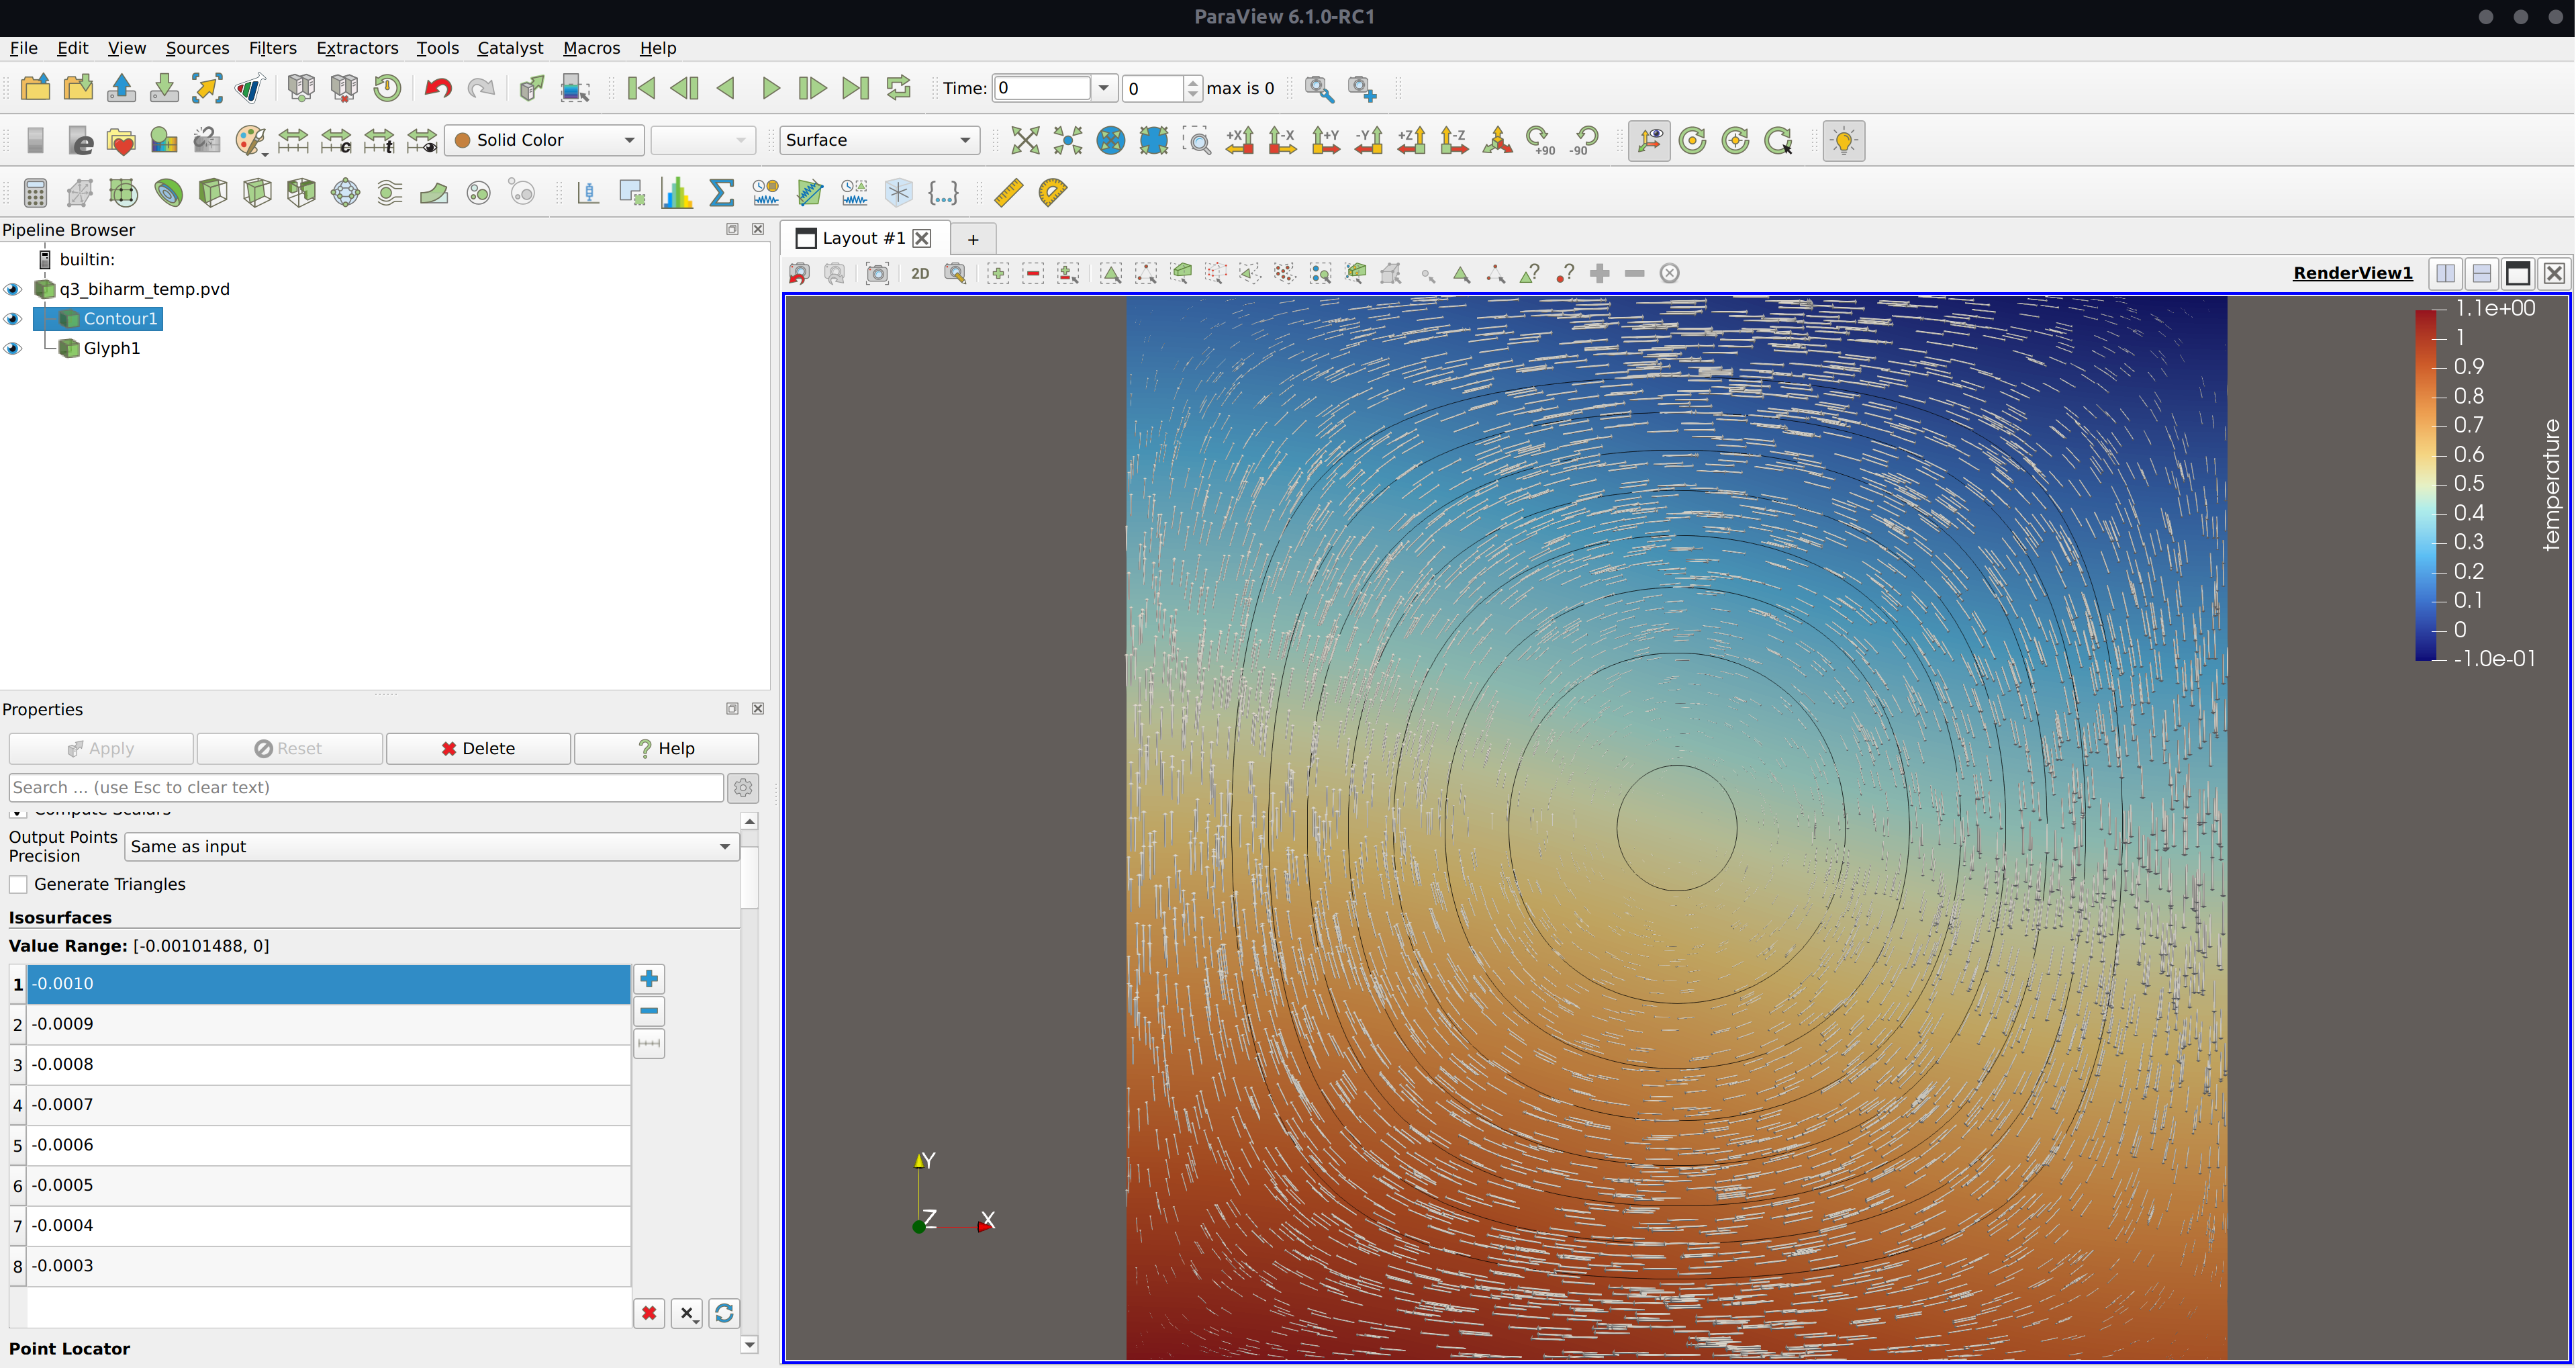
\includegraphics[width=1\textwidth]{./biharm_temp/result/q3_biharm_temp.png}
    \caption{The solution of this temperature-driven biharmonic problem. Looks like a Jean's instability about to form or Rayleigh-Benard convection, basically a sinusoidal perturbation in the temperature field that drives a flow.}
    \label{fig:q3_biharm_temp}
\end{figure}


\newpage
\section{Question 4: convection.py}

WE are asked to solved a convection problem by conbining the biharmonic solver and the heat.py solver. We need to solve Equations above with the boundary conditions specified in the problem statement

\begin{equation}
    \begin{array}{rl}{T(x,0,t)=1}&{{}T(x,1,t)=0}\\
{\frac{\partial T}{\partial x}(0,y,t)=0}&{{}\frac{\partial T}{\partial x}(1,y,t)=0}\\
{\omega=0}&{{}\psi=0\quad\mathrm{on}~\partial\Omega}\end{array}
\end{equation}
with the initial condition
\begin{equation}
    T(x,y,0) = 1 - y + A \cos(\pi x)
\end{equation}

\subsection{(a) $Ra = 10^2$}

Coding this up in firedrake is fairly simple with the following weak form
\begin{verbatim}
F_T = (
inner(T_dot, T_t)
+ inner(dot(v_flow, grad(T)), T_t)
+ (1 / Ra) * inner(grad(T), grad(T_t))
) * dx
F_omega = inner(grad(omega_t), grad(omega)) * dx - omega_t * T.dx(0) * dx
F_psi = inner(grad(psi_t), grad(psi)) * dx - psi_t * omega * dx
\end{verbatim}


with the boundary conditions 
\begin{verbatim}
    bcs = [
    DirichletBC(ME.sub(0), Constant(1.0), 3),  # T=1 bottom
    DirichletBC(ME.sub(0), Constant(0.0), 4),  # T=0 top
    DirichletBC(ME.sub(1), Constant(0.0), "on_boundary"),  # omega=0
    DirichletBC(ME.sub(2), Constant(0.0), "on_boundary"),  # psi=0
]
\end{verbatim}
and also the initial conditions
\begin{verbatim}
u.subfunctions[0].interpolate((1 - y) + Constant(0.1) * cos(pi * x))
u.subfunctions[1].interpolate(Constant(0.0))
u.subfunctions[2].interpolate(Constant(0.0))
\end{verbatim}

\begin{figure}
    \centering
    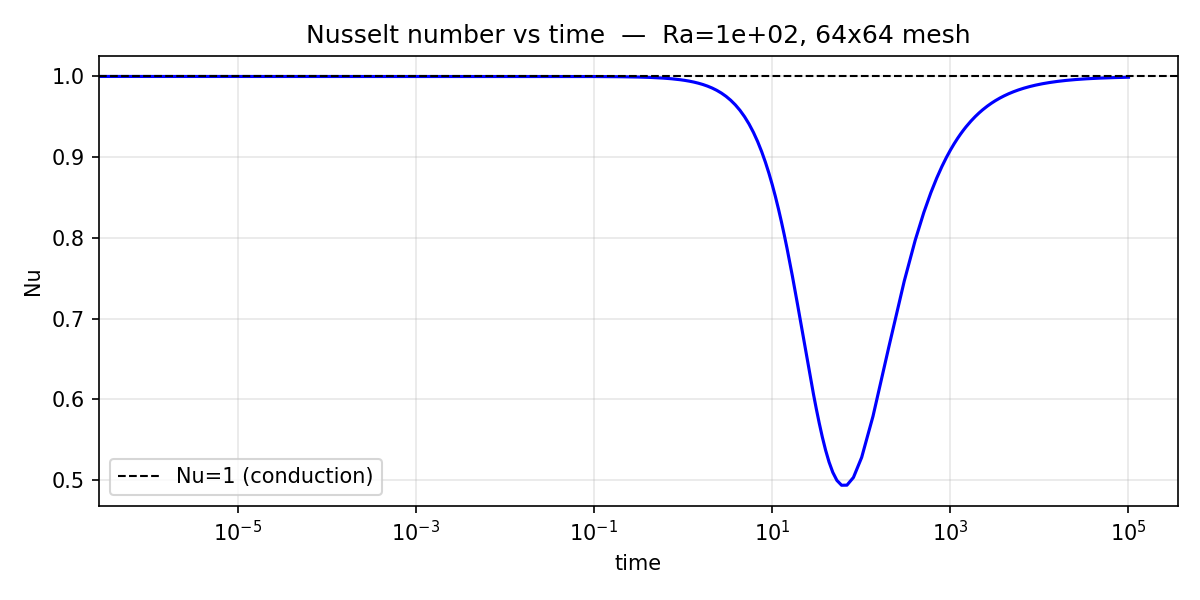
\includegraphics[width=1\textwidth]{./q4a_result/Nu_vs_time_Ra1e2_N64.png}
    \caption{The value of the Nusselt number over time for $Ra = 10^2$ on a 64x64 mesh. We see that the system reaches a steady state where Nu is approximately 1, after dipping to 0.5 near 10 and rises back to 1. This is consistent with the fact that $Ra = 10^2$ is below the critical Rayleigh number for convection, so the system is stable and heat is transferred primarily through conduction, which corresponds to Nu = 1. The initial dip in Nu could be due to the initial perturbation in the temperature field, but as the system evolves, it settles back to the conductive state.}
    \label{fig:q4a_Ra1e2}
\end{figure}

\subsection{(b) $Ra = 10^4, 10^5, 10^6$}

Increasing the Rayleigh number to $10^4, 10^5, 10^6$ will lead to more vigorous convection. We expect to see the Nusselt number increase significantly above 1, indicating that convection is enhancing heat transfer. I messed around with the timestep size since it was running quate slowly.

Here is the plot of Nu vs time for these three Rayleigh numbers, which shows that as we increase $Ra$, the Nusselt number increases significantly above 1, indicating stronger convection and enhanced heat transfer. Then it goes to a negative value, which is interesting and could be due to the initial conditions or the transient behavior of the system as it transitions to a convective state.  


Based on the resuslts below, however, we see that by $t = 10^5$ they all seem to try to converge to Nu = 1, which is unexpected since we should see some increase in Nu due to convection. Maybe for these choices of $Ra$, the system is still close to the critical Rayleigh number for convection, and the flow is not fully developed, which could explain why Nu is not increasing significantly above 1. Or We would have to run for much longer to see the fully developed convection and the increase in Nu, which is not feasable on my pc.

In fact, the plot for $Ra = 10^6$  was cut short, hence it does not evolve to $t = 10^5$.

\begin{figure}
    \centering
    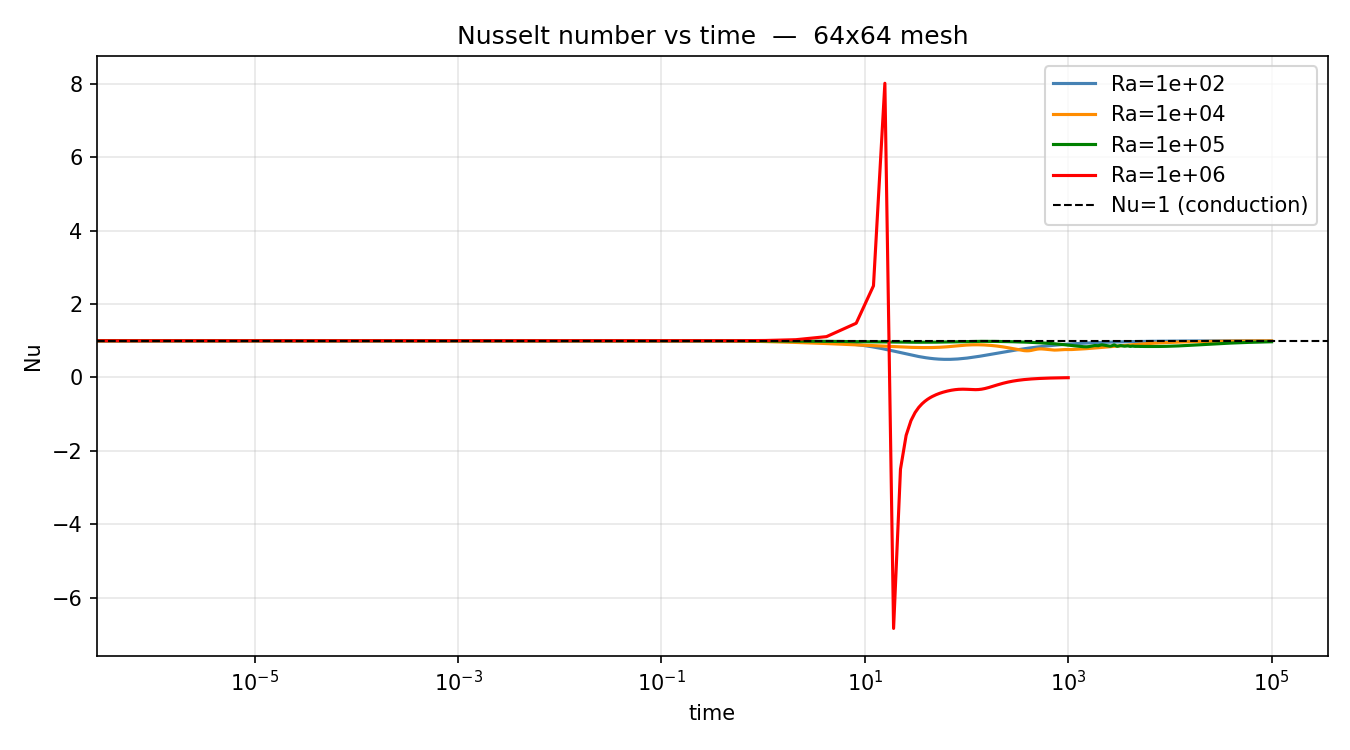
\includegraphics[width=0.8\textwidth]{./Nu_vs_time_combined_q4ab.png}
    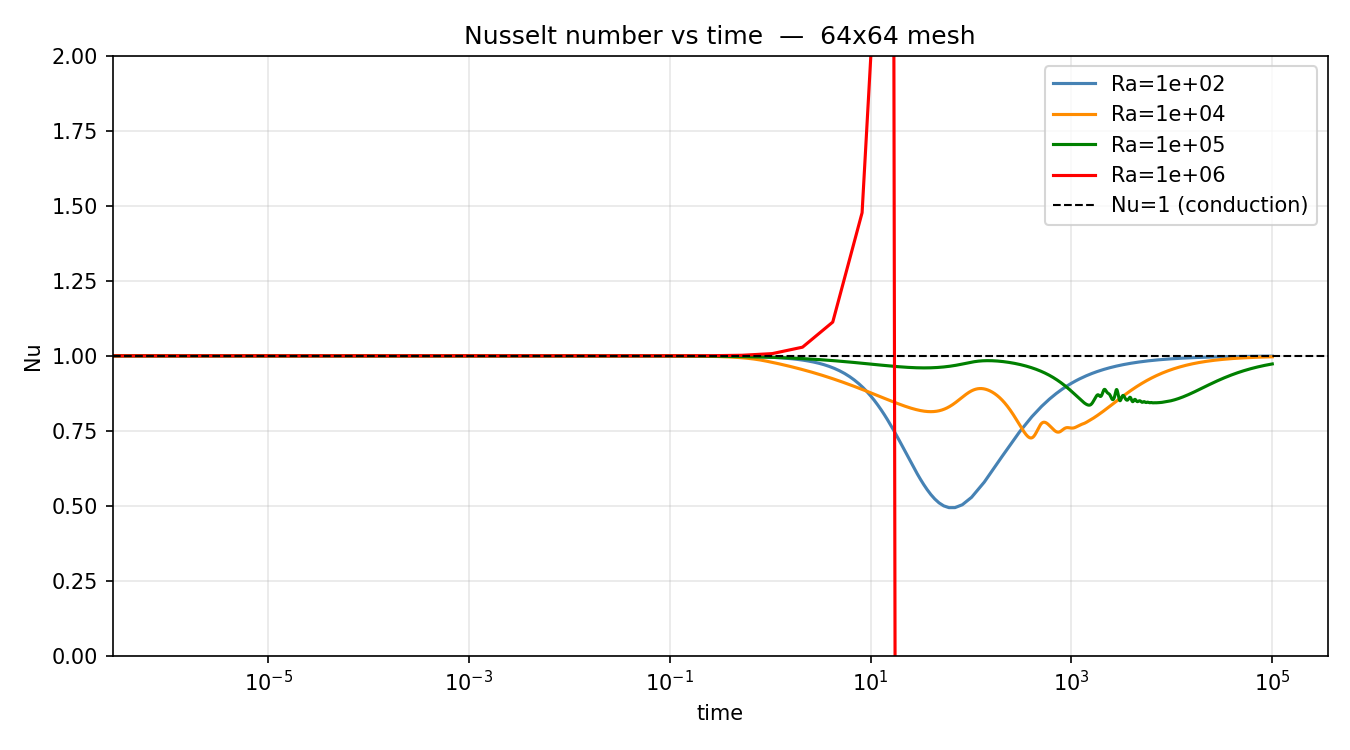
\includegraphics[width=1\textwidth]{./Nu_vs_time_combined_q4ab_zoomed.png}
    \caption{The value of the Nu over time for $Ra = 10^2, 10^4, 10^5, 10^6$ on a 64x64 mesh. We see that as we increase $Ra$, the Nusselt number over time changes in shape. the initial dip in Nu shifts to later times, and the dip decreases. The wiggles in the solution also become more pronounced as we increase $Ra$, which could be due to the more vigorous convection and the complex flow patterns that develop at higher Rayleigh numbers. For $Ra = 10^2$, the system reaches a steady state where Nu is approximately 1, which is consistent with the fact that $Ra = 10^2$ is below the critical Rayleigh number for convection, so the system is stable and heat is transferred primarily through conduction. For $Ra = 10^6$, there is a sharp rise followed by a dip to negative values, which could be due to the initial conditions or the transient behavior of the system as it transitions to a convective state. The negative values of Nu could indicate that there are regions in the flow where heat is being transferred in the opposite direction, which can happen in complex convective flows. This run (red line) is also very slow.}
    \label{fig:q4a_Ra1e2}
\end{figure}

\newpage
\subsection{(c) $Ra = 10^4$ for $N = 16, 32, 64, 128$}

\begin{figure}
    \centering
    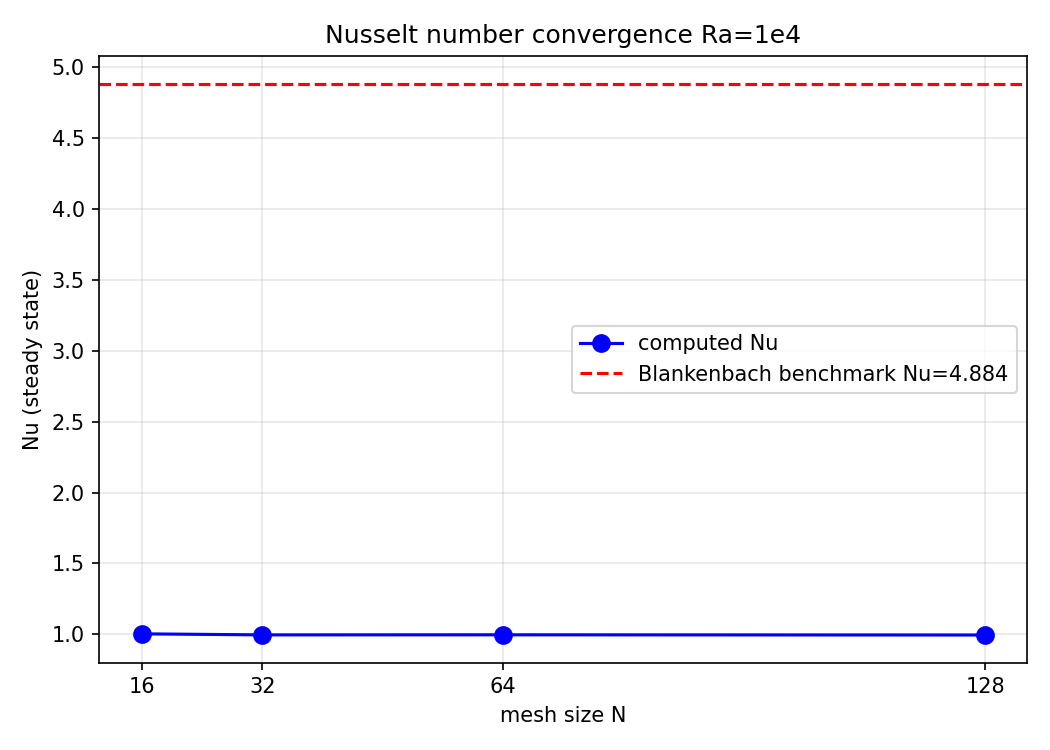
\includegraphics[width=1\textwidth]{./Nu_vs_meshsize_Ra1e4.png}
    \caption{The end value of the Nusselt number for $Ra = 10^4$ as a function of mesh size. For some reason, Nu is relatively stable at 1.0 across all mesh sizes, which is unexpected since we should see some increase in Nu due to convection.}
    \label{fig:q4a_Ra1e2}
\end{figure}

Here is Nu as a function of time for $Ra = 10^4$ for different mesh sizes. 


\begin{figure}
    \centering
    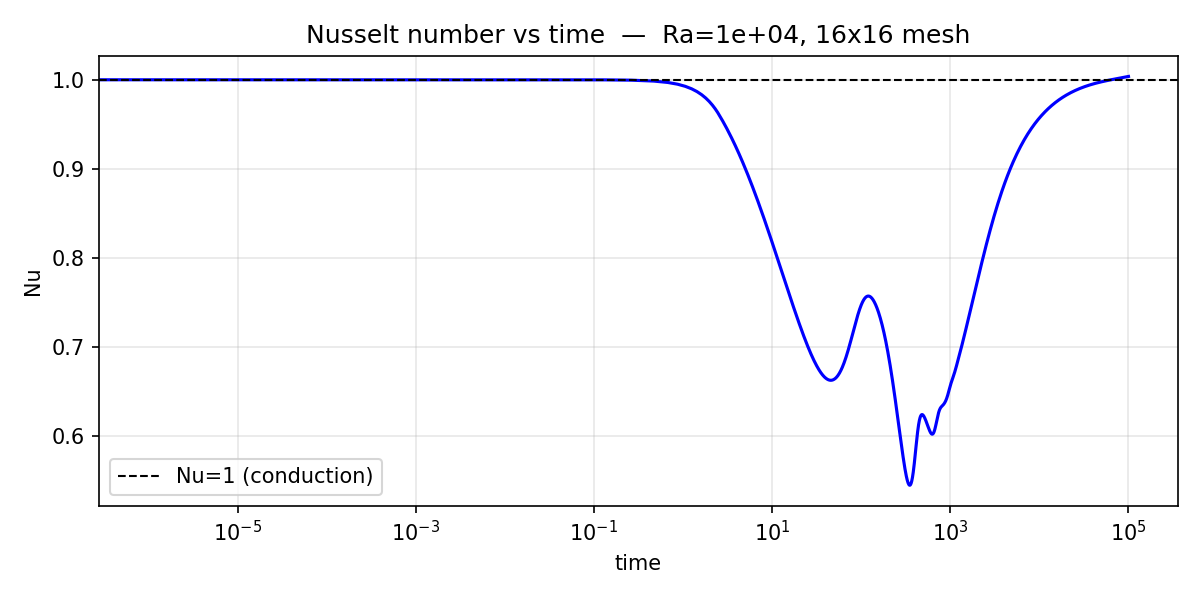
\includegraphics[width=0.5\textwidth]{./q4c_result/Nu_vs_time_Ra1e4_N16.png}
    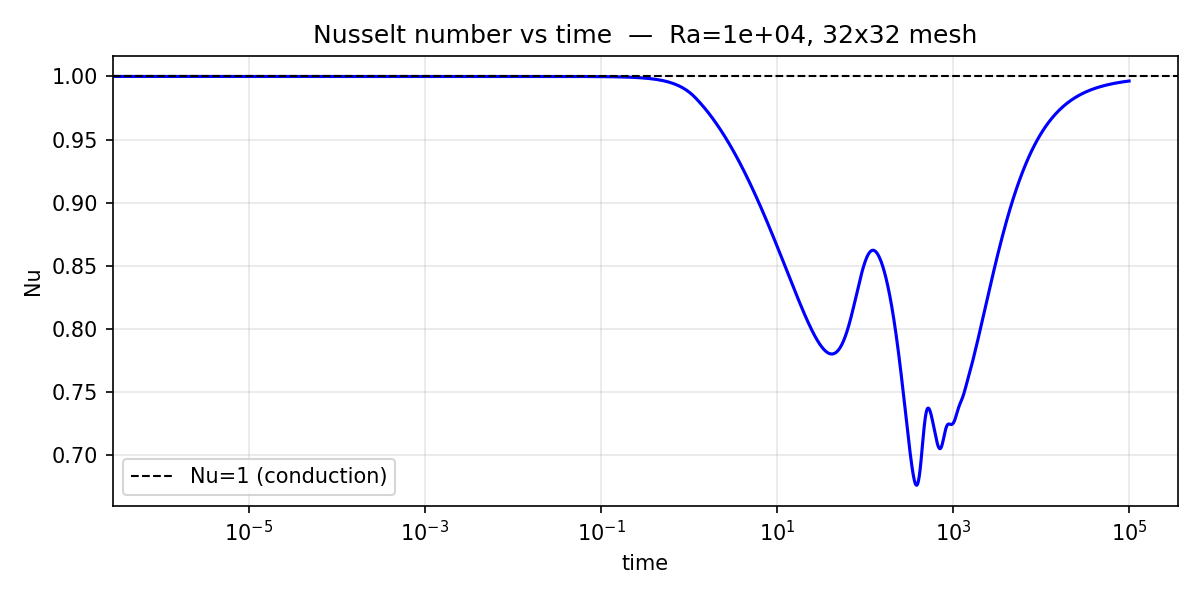
\includegraphics[width=0.5\textwidth]{./q4c_result/Nu_vs_time_Ra1e4_N32.png}
    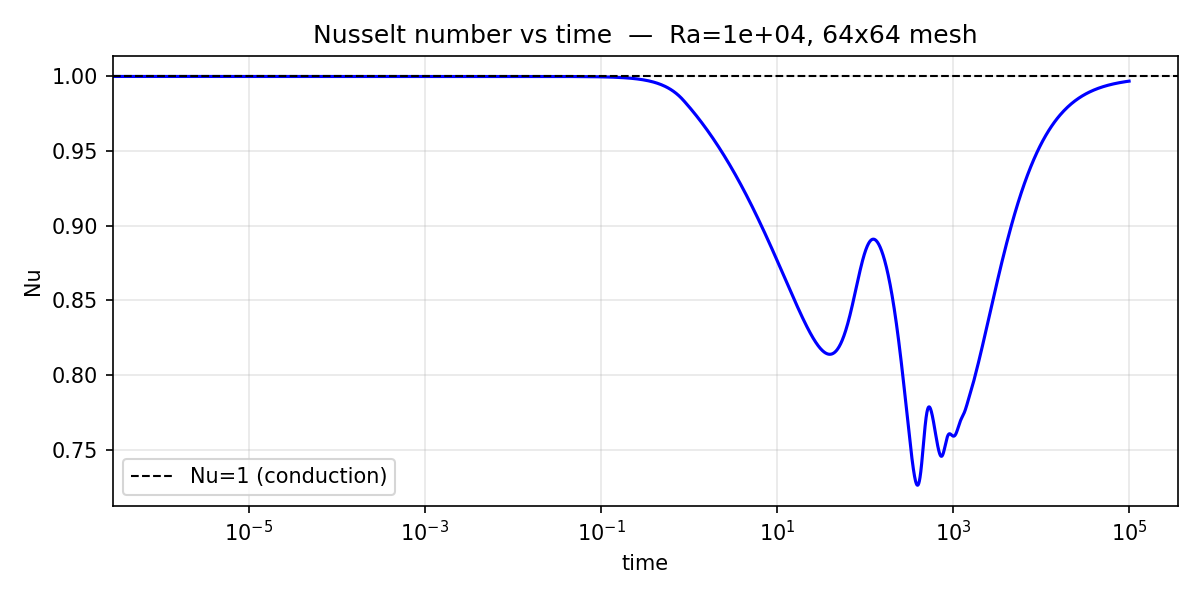
\includegraphics[width=0.5\textwidth]{./q4c_result/Nu_vs_time_Ra1e4_N64.png}
    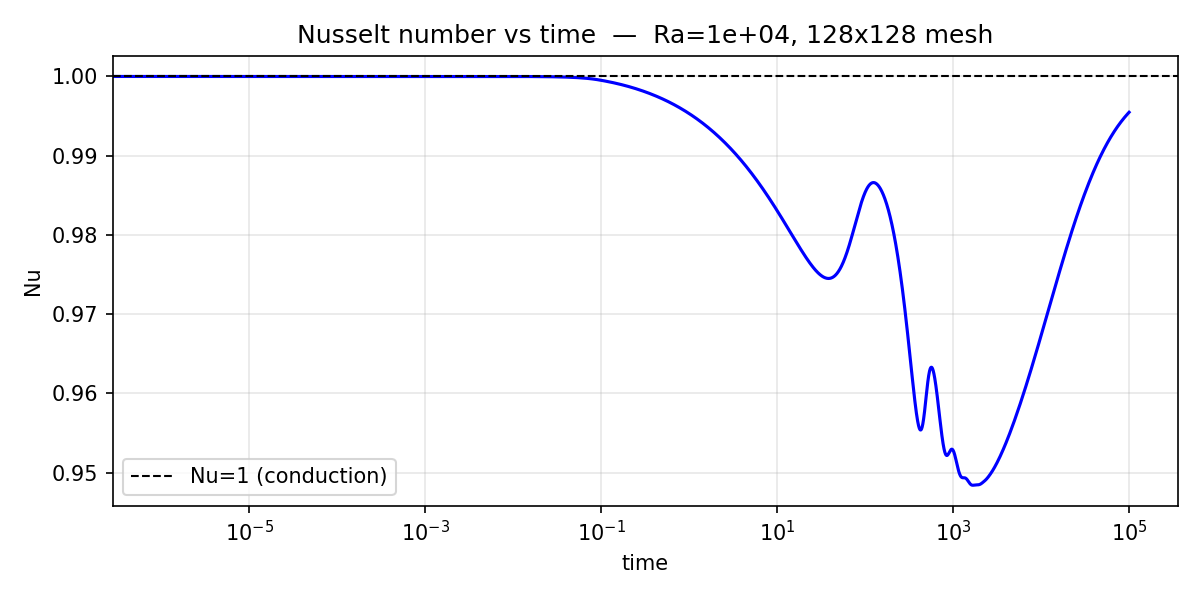
\includegraphics[width=0.5\textwidth]{./q4c_result/Nu_vs_time_Ra1e4_N128.png}
    \caption{The value of the Nusselt number over time for $Ra = 10^4$ for different mesh sizes. We see that as we increase the mesh size, the Nusselt number seems to be unchanged, apart from the feature past 1e3.}
    \label{fig:q4a_Ra1e2}
\end{figure}

The exepected behavior of changing the mesh size is that as we increase the mesh size, we should see a more accurate representation of the flow and temperature fields, which could lead to a more accurate calculation of the Nusselt number. Nu = 4.884 would I think be a special case for this problem, and we should see the Nusselt number converge to this value as we refine the mesh. However, in our results, we see that the Nusselt number is relatively stable at around 1.0 across all mesh sizes, which is unexpected since we should see some increase in Nu due to convection. 

Maybe for this choice of $Ra = 10^4$, the system is still close to the critical Rayleigh number for convection, and the flow is not fully developed, which could explain why Nu is not increasing significantly above 1.0.

\end{document}